% Copyright (c) 2008-2009 solvethis
% Copyright (c) 2010-2016,2018-2019,2021 Casper Ti. Vector
% Copyright (c) 2021 Kurapica

%*********************************************************************
% 四川师范大学硕士研究生学位论文模板
% 2022/12/15 v1.0.0
%
% 重要提示:
%   1. 当前模版参考2015年1月22日发布在四川师范大学研究生院官网的“四川师范大学博士、硕士学位论文撰写打印要求及格式范本”.
%   2. 当前版本基于 Macos 制作并测试通过
%   3. 请使用UTF-8编码,XeLaTeX方式编译
%   4. 请仔细阅读用户文档
%   5. 修改、使用、发布本文档类请务必遵循LaTeX Project Public License和知识共享4.0
%   6. 如有疑问请联系作者 图灵的猫 turingscat@126.com Qid:TuringsCat
% 免责声明:此模版制作初衷是为四川师范大学偏微分方程与数学物理团队提供更高效的硕士研究生学位论文模版。
% 对于提供的所有内容,不完全保证所有内容的完整性、准确性和及时性,本模版仅供学习、交流和分享用途,只供参考。
% 此模版一经使用,即表示您已经接受上述声明!需自行承担一切风险与责任。
% 以上声明内容最终解释权在法律允许内归作者所有。
%*********************************************************************

%======================== 排序环境宏包 ===============================%
\usepackage{enumerate}
\usepackage{xcolor}
\usepackage{./setup/ccmap}     %实现浮动对象的双语说明的宏包
\usepackage{floatrow}  %用于调整图片或表格的位置
\floatsetup[table]{capposition=top}
\floatsetup[figure]{capposition=bottom}
\usepackage{subfigure} %Latex插入子图宏包
\usepackage{float} %限制浮动的位置在当前位置[H]
\usepackage{multirow}% 绘制多行表格
\usepackage{booktabs}
% \usepackage{hyperref}% 实现交叉引用自动跳转
% \hypersetup{
% colorlinks=true,
% linkcolor=black
% }
\usepackage[hidelinks]{hyperref}
%======================== 数学公式相关宏包 ===============================%
\usepackage{bm}         % 处理数学公式中的黑斜体的宏包
\usepackage{dsfont}   
% \usepackage{latexsym}   %使用不同的符号字体宏包
\usepackage{amsmath}    % AMSLaTeX宏包 用来排出更加漂亮的公式
\usepackage{amssymb}    % AMSLaTeX宏包 用来排出更加漂亮的公式
\usepackage{mathrsfs}  % 不同于\mathcal or \mathfrak 之类的英文花体字体
\usepackage[amsmath,thmmarks]{ntheorem} % 定理类环境宏包,其中 amsmath 选项
                                        % 用来兼容 AMS LaTeX 的宏包  
%framed: 需要边框时,须调用framed宏包和pstricks宏包;
%thmmarks: 需要有结束符时;
%thref,hyperref: 需要有交叉引用与hyperref 宏包时.                               
\usepackage{subeqnarray} %多个子方程(1-1a)(1-1b)
            %范例
            %\begin{subeqnarray}
            %\label{eqw} \slabel{eq0}
            % x & = & a \times b \\
            %\slabel{eq1}
            % & = & z + t\\
            %\slabel{eq2}
            % & = & z + t
            %\end{subeqnarray}

%============================表格支持宏包=================================%
\usepackage{rotating}   % 用法 \begin{sidewaystable}....\end{sidewaystable}
                        % 即可旋转表格
\usepackage{longtable}  % 支持长表格
\usepackage{tabls}
\usepackage{multirow}   % 表格多行合并, 矩阵的边注
\usepackage{colortbl}   % 彩色表格
\usepackage{dcolumn}    % 让表格中将小数点对齐
\usepackage{hhline}     % 在表格中用 \hhline 得到的结果就如同\hline
                        % 或 \hline\hline,当然在和垂直线的交叉处会有所不同.
\usepackage{./setup/slashbox}   % 可在表格的单元格中画上一斜线.  
\usepackage{array}

%=========================== 特殊文本元素宏包 ==============================%
\usepackage{nicefrac}   % 在正文文本中排版分式时,可以用它来得到较好的排版效果.
\usepackage{units}      % 基于 nicefrac 宏包,提供对计量单位比较美观的排版效果.
\usepackage{soul}       % 支持对单词加上下划线或其每个字母在一定的宽度内均匀散布
\usepackage{altfont}    % 使用该宏包, 可以在一个宏包中使用多种不同的字体,
                        % 包括PSNFSS 和 MFNFSS
\usepackage{a0size}     %自由定义字号,在后面“字号设置”中可设置到107pt 为止的大字体

%=============================== 其他宏包 ==================================%
% \usepackage{epstopdf}   % 将eps文件转换为pdf
% \usepackage{prelim2e}   % 可以在每页页脚下方标记出本文档的版本信息等
% \usepackage{mathptmx}   % 如果您的 TeX 系统可用,请使用 Times 字体
\usepackage{graphicx}     %插入浮动图片的宏包
\usepackage{marvosym}     %小信封
\usepackage{color}        %LaTeX中设置字体颜色
\usepackage{appendix}     %在latex文件中加入附录的依赖
\usepackage{times}        %提供Time New Roman字体

\usepackage[a4paper,left=25mm,right=25mm,top=30mm,bottom=25mm,headheight=23cm,headsep=2mm,footskip=7mm]{geometry}
%设置行间距,这是粗略设定,大体与20pt无差距
% \linespread{1.38}\selectfont%1.38 1.25
%也可使用setspace宏包,不过貌似其1.5倍行距与word的不同
%\usepackage{setspace}
%\onehalfspacing
%实在觉得不妥,干脆直接指定行距为20pt了,必须在begin{document}之后使用
%\baselineskip=20pt
\sloppy
% LaTeX 总是尽可能产生最好的断行效果,如果断行无法达到 LaTeX 要求的标准,
%就会是这一行在段落的右侧溢出,同时报告"overfull hbox"消息.
%可以使用\sloppy命令降低标准.\fussy恢复为缺省状态.


%+++++++++++++++++++++++页眉页脚++++++++++++++++++++++++++++++
%+++++++++++++++++++++++++++++++++++++++++++++++++++++++++++++
%版式设置宏包,设置页眉页脚
\usepackage{fancyhdr}
\pagestyle{fancy}
\renewcommand{\chaptermark}[1]{\markboth{\thechapter \ #1}{}}            % \chaptermark{}会在使用\chapter{}命令时自动调用,即每次设置章节的时候,都会同时调用 \chaptermark{}。

\renewcommand{\sectionmark}[1]{\markright{\thesection \ #1}{}}            % 同理,\sectionmark{}会在使用\section{}命令时调用。
\fancypagestyle{plain}{
\fancyhf{}
\fancyfoot[EL]{{\zihao{-5}\songti \thepage}}
\fancyfoot[OR]{{\zihao{-5}\songti \thepage}}
\fancyhead[EC]{{\zihao{-5}\songti 四川师范大学硕士学位论文}}
% \fancyhead[EC]{{\zihao{-5}\songti 四川师范大学博士学位论文}}
\fancyhead[OC]{{\zihao{-5}\songti \leftmark}}
\renewcommand{\headrulewidth}{0.4pt}
}
% \pagestyle{plain}


%+++++++++++++++++++++++目录环境设置++++++++++++++++++++++++++
%+++++++++++++++++++++++++++++++++++++++++++++++++++++++++++++

%目录改为目次
\renewcommand{\contentsname}{目录}

\usepackage[nottoc]{tocbibind} %自动将参考文献、索引、插图等标题及其页码加入目录,也可禁止某些项进入
%也就不用 \addcontentsline{toc}{chapter}{\listfigurename} 和这个 \addcontentsline{toc}{chapter}{参考文献}
\usepackage{titletoc}
%\titlecontents{标题名}[左间距]{标题格式}{标题标志}{无序号标题}{指引线与页码}[下间距]
\titlecontents{chapter}[0em]{\zihao{-4}\songti\addvspace{5pt}}{\thecontentslabel\hspace{1em}}{}{\titlerule*[0.5pc]{.}\contentspage}
\titlecontents{section}[1.8em]{\zihao{-4}\songti\addvspace{5pt}}{\thecontentslabel\hspace{0.5em}}{}{\titlerule*[0.5pc]{.}\contentspage}
\titlecontents{subsection}[3.5em]{\zihao{-4}\songti\addvspace{5pt}}{\thecontentslabel\hspace{0.5em}}{}{\titlerule*[0.5pc]{.}\contentspage}


%+++++++++++++++++++++++图表设置++++++++++++++++++++++++++++++
%+++++++++++++++++++++++++++++++++++++++++++++++++++++++++++++
\usepackage{epsfig}

%图表混合目录
\makeatletter \renewcommand{\ext@table}{lof} \makeatother
\renewcommand{\listfigurename}{插图和附表清单}
\titlecontents{figure}[0em]{\zihao{-4}\songti\addvspace{5pt}}{图~\thecontentslabel\hspace{1em}}{}{\titlerule*[0.5pc]{.}\contentspage}
\titlecontents{table}[0em]{\zihao{-4}\songti\addvspace{5pt}}{表~\thecontentslabel\hspace{1em}}{}{\titlerule*[0.5pc]{.}\contentspage}

%图标标题设定
\usepackage[font=small,labelfont=bf,textfont=bf,labelsep=space,belowskip=-1em]{caption}

%图形处理宏包overpic, 用来在图片上放置文字
\usepackage{overpic}


%+++++++++++++++++++++++摘要环境++++++++++++++++++++++++++++++
%+++++++++++++++++++++++++++++++++++++++++++++++++++++++++++++

%中文摘要环境
\newenvironment{ChineseAbstract}[1][]{
\songti\chapter[摘要]{\thesicnutitlec}

\centerline{{\heiti \bf 专业:\thesicnumajorc }{\heiti }}
\centerline{}
\centerline{{\heiti\bf 研究生:}~~{\kaishu \thesicnuauthorc}\qquad{\heiti \bf 指导教师:}~~{\kaishu \thesicnusupervisorc~#1}}
\list{}{
\itemindent=2em
\listparindent=2em
\itemsep=0pt
\leftmargin=0pt
\rightmargin=0pt
\labelsep=0.5em
\labelwidth=2em
\parsep=0pt
}
\item
\item
}
{\endlist}

%英文摘要环境
\newenvironment{EnglishAbstract}{
\songti\chapter[ABSTRACT]{\thesicnutitlee}

\centerline{{\bf Major:}~~{\bf\thesicnumajore}}
\centerline{}
\centerline{{\bf Master:}~~{\thesicnuauthore}\qquad{\bf Supervisor:}~~{\thesicnusupervisore}}
\list{}{
\itemindent=2em
\listparindent=2em
\itemsep=0pt
\leftmargin=0pt
\rightmargin=0pt
\labelsep=0.5em
\labelwidth=2em
\parsep=0pt
}
\item
\item
}
{\endlist}


%+++++++++++++++++++++++参考文献++++++++++++++++++++++++++++++
%+++++++++++++++++++++++++++++++++++++++++++++++++++++++++++++
%BibTeX参考文献支持宏包
\usepackage{texnames}   %用于显示BibTeX
\usepackage[numbers,sort&compress]{natbib}
% %下面的命令\citep将参考文献以上标形式出现
% \let\oldcitep\citep
% \newcommand{\citen}[2][]{\textsuperscript{\oldcitep{#2}#1}}
% \renewcommand{\citep}{\citen}
% \usepackage[superscript,nomove]{cite} %上标引用

%调整条目间距离
\bibsep=0pt
%字体命令
\renewcommand{\bibfont}{\zihao{5}\songti}

%+++++++++++++++++++++++脚注格式++++++++++++++++++++++++++++++
%+++++++++++++++++++++++++++++++++++++++++++++++++++++++++++++
%脚注格式设定
\usepackage{pifont}
\renewcommand\thefootnote{\ding{\numexpr171+\value{footnote}}}


%+++++++++++++++++++++++题名页环境++++++++++++++++++++++++++++
%+++++++++++++++++++++++++++++++++++++++++++++++++++++++++++++
%题名页支持宏包
\usepackage{ulem}
\usepackage{ifthen}
%题名页页定义命令
%论文作者中文名
\newcommand{\thesicnuauthorc}{刘洋}
\newcommand{\SiCNUAuthorC}[1]{\renewcommand{\thesicnuauthorc}{#1}}
%论文作者英文名
\newcommand{\thesicnuauthore}{Liu Yang}
\newcommand{\SiCNUAuthorE}[1]{\renewcommand{\thesicnuauthore}{#1}}
%指导教师中文名
\newcommand{\thesicnusupervisorc}{冉茂华}
\newcommand{\SiCNUSupervisorC}[1]{
\newlength{\supervisorclength}
\settowidth{\supervisorclength}{#1}
\ifthenelse{\lengthtest{\supervisorclength = 0em}}
    {\renewcommand{\thesicnusupervisorc}{\hspace{3em}}}
    {\renewcommand{\thesicnusupervisorc}{#1}}
}
%指导教师英文名
\newcommand{\thesicnusupervisore}{Ran Maohua}
\newcommand{\SiCNUSupervisorE}[1]{\renewcommand{\thesicnusupervisore}{#1}}
%专业名称中文
\newcommand{\thesicnumajorc}{偏微分方程与数学物理}
\newcommand{\SiCNUMajorC}[1]{\renewcommand{\thesicnumajorc}{#1}}
%专业名称英文
\newcommand{\thesicnumajore}{Partial Differential Equations and Mathematical Physics}
\newcommand{\SiCNUMajorE}[1]{\renewcommand{\thesicnumajore}{#1}}
%学号
\newcommand{\thesicnunumber}{20210801068}
\newcommand{\SiCNUNumber}[1]{
\newlength{\numberlength}
\settowidth{\numberlength}{#1}
\newlength{\numberlengthundefinde}
%单位代码
\settowidth{\numberlengthundefinde}{10636}
\ifthenelse{\lengthtest{\numberlength = 0em} \or \lengthtest{\numberlength < \numberlengthundefinde}}
{\renewcommand{\thesicnunumber}{\qquad\qquad}}
{\renewcommand{\thesicnunumber}{#1}}
}
%分类号
\newcommand{\thesicnuclass}{\zihao{5} O241.82}
\newcommand{\SiCNUClass}[1]{\renewcommand{\thesicnuclass}{#1}}
%密级
\newcommand{\thesicnusecret}{\zihao{5} 公开}
\newcommand{\SiCNUSecret}[1]{\renewcommand{\thesicnusecret}{#1}}
%研究方向
\newcommand{\thesicnuresearch}{偏微分方程数值解}
\newcommand{\SiCNUResearch}[1]{\renewcommand{\thesicnuresearch}{#1}}
% 所在学院
\newcommand{\thesicnucollege}{数学科学学院}
\newcommand{\SiCNUCollege}[1]{\renewcommand{\thesicnucollege}{#1}}
%论文中文题目
\newcommand{\thesicnutitlec}{二维分数阶非线性薛定谔波方程的数值方法与守恒性质研究}
%论文中文分行题目
\newcommand{\thesicnutitleca}{二维分数阶非线性薛定谔波方程的}
\newcommand{\thesicnutitlecb}{数值方法与守恒性质研究}
\newcommand{\SiCNUTitleC}[2][]{
\newlength{\titleca}
\settowidth{\titleca}{#2}
\newlength{\titlecb}
\settowidth{\titlecb}{#1}
\ifthenelse{\lengthtest{\titleca > 18em}}
    {\renewcommand{\thesicnutitleca}{标题过长, 请用可选参数}}%每行字数不超过~18
    {\renewcommand{\thesicnutitleca}{#2}}
\ifthenelse{\lengthtest{\titlecb > 18em}}
    {\renewcommand{\thesicnutitlecb}{标题过长, 请缩短标题}}
    {\renewcommand{\thesicnutitlecb}{#1}}
\ifthenelse{\lengthtest{\titleca > 18em} \and \lengthtest{\titlecb > 18em}}
    {\renewcommand{\thesicnutitleca}{标题过长, 请缩短标题}\renewcommand{\thesicnutitlecb}{标题过长, 请缩短标题}}
    {}
\renewcommand{\thesicnutitlec}{#2 #1}
\ifthenelse{\equal{#2}{}}
    {\renewcommand{\thesicnutitlec}{\hspace{17em}}}
    {}
}
%论文英文题目
\newcommand{\thesicnutitlee}{Numerical Methods and Conservation Properties for the Two-Dimensional Fractional Nonlinear Schr{\"o}dinger Wave Equation}
%论文英文分行题目
\newcommand{\thesicnutitleea}{Numerical Methods and Conservation Properties}
\newcommand{\thesicnutitleeb}{for the Two-Dimensional Fractional Nonlinear}
\newcommand{\thesicnutitleec}{Schr{\"o}dinger Wave Equation}
\newcommand{\SiCNUTitleE}[3][]{
\newlength{\titleea}
\settowidth{\titleea}{#2}
\newlength{\titleeb}
\settowidth{\titleeb}{#1}
\newlength{\titleec}
\settowidth{\titleec}{#3}
\ifthenelse{\lengthtest{\titleea > 18em}}
    {\renewcommand{\thesicnutitleea}{标题过长, 请用可选参数}}%每行字数不超过~18
    {\renewcommand{\thesicnutitleea}{#1}}
\ifthenelse{\lengthtest{\titleeb > 18em}}
    {\renewcommand{\thesicnutitleeb}{标题过长, 请缩短标题}}
    {\renewcommand{\thesicnutitleeb}{#2}}
\ifthenelse{\lengthtest{\titleec > 18em}}
    {\renewcommand{\thesicnutitleec}{标题过长, 请缩短标题}}
    {\renewcommand{\thesicnutitleec}{#3}}
\ifthenelse{\lengthtest{\titleea > 18em} \and \lengthtest{\titleeb > 18em}\and \lengthtest{\titleec > 18em}}
    {\renewcommand{\thesicnutitleea}{标题过长, 请缩短标题}\renewcommand{\thesicnutitleeb}{标题过长, 请缩短标题}\renewcommand{\thesicnutitleec}{标题过长, 请缩短标题}}
    {}
\renewcommand{\thesicnutitlee}{#3#2 #1}
}

%论文提交日期
\newcommand{\thesicnudateofsubmit}{2024年5月20日\ \ \ \ \ \ \ \ }
\newcommand{\SiCNUDateOfSubmit}[1]{\renewcommand{\thesicnudateofsubmit}{#1}}
%论文答辩日期
\newcommand{\thesicnudateofdefence}{2024年5月20日\ \ \ \ \ \ \ \ }
\newcommand{\SiCNUDateOfDefence}[1]{\renewcommand{\thesicnudateofdefence}{#1}}
%\newcommand{}{}
%\newcommand{}[1]{\renewcommand{}{#1}}


\newcommand{\SiCNUMakeTitle}{
\begin{titlepage}
  \newlength{\Mycode}
  \settowidth{\Mycode}{学\qquad 号: \thesicnunumber}
  \newlength{\MyCT}
  \settowidth{\MyCT}{\zihao{3}\bfseries\songti 中文论文题目: }
  \begin{center}
  \vspace*{1em}  
  \vspace*{0.5em}
    \begin{minipage}[t]{14em}
      分类号: \uline{\hfill \mbox{\thesicnuclass} \hfill}\\[0.4em]
      密\quad 级: \uline{\hfill \mbox{\thesicnusecret} \hfill}
    \end{minipage}
    \hfill
    \begin{minipage}[t]{\Mycode}
      单位代码: \uline{\hfill 10636 \hfill}\\[0.4em]
      学\qquad 号: \uline{\thesicnunumber}
    \end{minipage}
    \par \vspace{1em}
    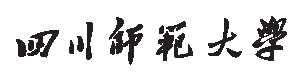
\includegraphics[width=9cm]{setup/flage.eps}
    \par \vspace{1em}
    {\zihao{0}\bfseries\sffamily 硕\ 士\ 学\ 位\ 论\ 文}
    % {\zihao{0}\bfseries\sffamily 博\ 士\ 学\ 位\ 论\ 文} 
    % {\zihao{0}\bfseries\sffamily 专\ 业\ 学\ 位\ 硕\ 士\ 论\ 文}
    \par \vspace{1em}
    
\includegraphics[width=3cm]{setup/logo.eps}
    \par \vspace{2em}
    \renewcommand{\ULthickness}{0.6pt}\setlength{\ULdepth}{4pt}
    {\zihao{3}\bfseries\songti 中文论文题目: }\uline{\hfill \zihao{-2}\bfseries\fangsong\mbox{\thesicnutitleca} \hfill}
    \par \vspace{0.5em}
    \hspace{\MyCT}\uline{\hfill\zihao{-2}\bfseries\fangsong\mbox{\thesicnutitlecb} \hfill}
    \par \vspace{0.5em}
    %   {\zihao{3}\bfseries\songti 英文论文题目: }\uline{\hfill\bfseries{\fontsize{16}{20}\selectfont\mbox{\thesicnutitleea}} \hfill}
    % \par \vspace{0.5em}
    % \hspace{\MyCT}\uline{\hfill\bfseries\textrm{\fontsize{16}{20}\selectfont\mbox{\thesicnutitleeb}} \hfill}
    % \par \vspace{0.5em}
    % \hspace{\MyCT}\uline{\hfill\bfseries\textrm{\fontsize{16}{20}\selectfont\mbox{\thesicnutitleec}} \hfill}
    % \par \vspace{2em}
    {\zihao{3}\bfseries\songti 英文论文题目: }\uline{\hfill{\fontsize{16}{20}\selectfont\mbox{\thesicnutitleea}} \hfill}
    \par \vspace{0.5em}
    \hspace{\MyCT}\uline{\hfill\textrm{\fontsize{16}{20}\selectfont\mbox{\thesicnutitleeb}} \hfill}
    \par \vspace{0.5em}
    \hspace{\MyCT}\uline{\hfill\textrm{\fontsize{16}{20}\selectfont\mbox{\thesicnutitleec}} \hfill}
    \par \vspace{2em}
    \begin{minipage}[t]{22em}
      \zihao{4}
      论文作者: \uline{\hfill\fangsong\mbox{\thesicnuauthorc}\hfill}\\[0.5em]
      指导教师: \uline{\hfill\fangsong\mbox{\thesicnusupervisorc}\hfill}\\[0.5em]
      专业名称: \uline{\hfill\fangsong\mbox{\thesicnumajorc}\hfill}\\[0.5em]
      研究方向: \uline{\hfill\fangsong\mbox{\thesicnuresearch}\hfill}\\[0.5em]
      所在学院: \uline{\hfill\fangsong\mbox{\thesicnucollege}\hfill}\\[0.5em]
      论文提交日期: \uline{\hfill\fangsong\mbox{\thesicnudateofsubmit}}\\
      论文答辩日期: \uline{\hfill\fangsong\mbox{\thesicnudateofdefence}}
      \par
    \end{minipage}
  \end{center}
\end{titlepage}
\thispagestyle{empty}
\cleardoublepage
}


%+++++++++++++++++++++++文体环境设置++++++++++++++++++++++++++
%+++++++++++++++++++++++++++++++++++++++++++++++++++++++++++++

\newcommand{\SiCNUfrontmatter}{
\frontmatter
\pagestyle{plain}
%改页码格式为大写罗马字体
\pagenumbering{Roman}
\renewcommand{\chaptermark}[1]{\markboth{ \ ##1}{}}%去掉页眉编号
%前一部分章节格式
\CTEXsetup[number={},nameformat={\zihao{-2}\songti},titleformat={\zihao{-2}\songti},
beforeskip={2em},afterskip={1em}]{chapter}
}

\newcommand{\SiCNUmainmatter}{
\mainmatter
%定制正文章节格式
\renewcommand{\chaptermark}[1]{\markboth{\thechapter \ ##1}{}}

\CTEXsetup[name={,},number={\arabic{chapter}},
format={\flushleft},nameformat={\zihao{3}\bf},%numberformat={},
aftername={~~},titleformat={\zihao{3}\bf},
beforeskip={1em},afterskip={0.5em}]{chapter}
\CTEXsetup[name={,},number={\arabic{chapter}.\arabic{section}},
format={\flushleft},nameformat={\zihao{4}\bf},%numberformat={},
aftername={~~},titleformat={\zihao{4}\bf},
beforeskip={0.5em},afterskip={0.5em}]{section}
\CTEXsetup[name={,},number={\arabic{chapter}.\arabic{section}.\arabic{subsection}},
format={\flushleft},nameformat={\zihao{-4}\bf},%numberformat={},
aftername={~~},titleformat={\zihao{-4}\heiti},
beforeskip={0em},afterskip={0em}]{subsection}
}

\newcommand{\SiCNUref}{
%参考文献章节格式
\CTEXsetup[number={},format={\center}]{chapter}
%参考文献字体, 使用natbib宏包时用其中命令修改
%\zihao{5}
}

\newcommand{\SiCNUappendix}{
\appendix
%附录章节格式
\CTEXsetup[name={附录,},number={\Alph{chapter}},format={\center}]{chapter}
\CTEXsetup[name={附录,},number={\Alph{chapter}.\arabic{section}},format={\center}]{section}
%附录页眉更改
\renewcommand{\chaptermark}[1]%
{\markboth{附录 \thechapter \ ##1}{}}
\zihao{-4}
}

\newcommand{\SiCNUbackmatter}{
\backmatter
%文后章节设置
\CTEXsetup[name={,},number={},format={\center}]{chapter}
%文后页码设置
% \renewcommand{\chaptermark}[1]{\markboth{\chaptername \ ##1}{}}
\renewcommand{\chaptermark}[1]{\markboth{ \ ##1}{}}
}

% 在校期间的科研成果
\newenvironment{mypaper}{
	\clearpage
	\phantomsection
	% \addcontentsline{toc}{section}{在校期间的科研成果}
	\ctexset{bibname={在校期间的科研成果}}
}



%+++++++++++++++++++++独创性声明++++++++++++++++++++++++++++%
%+++++++++++++++++++++++++++++++++++++++++++++++++++++++++++%
%下划线可自动换行宏包
\usepackage{CJKfntef}
% \renewcommand{\CJKunderline}{\color{black}}
\newcommand{\dcspace}{\hspace{0.5em}}

\newcommand{\OriginalCreationStatement}{
\vspace*{2.5em}
\centerline{\fangsong\zihao{-3}四川师范大学学位论文独创性声明}
\vspace*{1.5em}

本人声明:所呈交学位论文\CJKunderline{\dcspace\thesicnutitlec,\dcspace}是本人在导师\CJKunderline{\dcspace\thesicnusupervisorc\dcspace} 指导下,独立进行研究工作所取得的成果。除文中已经注明引用的内容外,本论文不含任何其他个人或集体已经发表或撰写过的作品或成果。对本文的研究做出重要贡献的个人和集体,均已在文中以明确方式标明。本声明的法律结果由本人承担。

本人承诺:已提交的学位论文电子版与论文纸本的内容一致。如因不符而引起的学术声誉上的损失由本人自负。
\vspace*{1.5em}

{\fangsong\zihao{4}学位论文作者:\hfill 签字日期:\quad\qquad 年 \qquad 月 \qquad 日}
\vspace{4em}

\centerline{\fangsong\zihao{-3}四川师范大学学位论文版权使用授权书}
\vspace*{1.5em}

本人同意所撰写学位论文的使用授权遵照学校的管理规定:

学校作为申请学位的条件之一,学位论文著作权拥有者须授权所在大学拥有学位论文的部分使用权,即:1)已获学位的研究生必须按学校规定提交印刷版和电子版学位论文,可以将学位论文的全部或部分内容编入有关数据库供检索;2)为教学、科研和学术交流目的,学校可以将公开的学位论文或解密后的学位论文作为资料在图书馆、资料室等场所或在有关网络上供阅读、浏览。
\vspace*{1.5em}

本人授权万方数据电子出版社将本学位论文收录到《中国学位论文全文数据库》,并通过网络向社会公众提供信息服务。同意按相关规定享受相关权益。 

(保密的学位论文在解密后适用本授权书)
\vspace*{1.5em}

\begin{minipage}[t]{14em}
  学位论文作者签名:\\[1.5em]
  签字日期:\qquad 年\qquad 月\qquad 日
\end{minipage}
\hfill
\begin{minipage}[t]{14em}
  导师签名:\\[1.5em]
  签字日期:\qquad 年\qquad 月\qquad 日
\end{minipage}
\thispagestyle{empty}
\fancyhf{}
\renewcommand{\headrulewidth}{0pt}
\cleardoublepage
}

%排序环境宏包
\usepackage{enumerate}
\usepackage[T1]{fontenc}%加粗所需宏包
\let\originaleqref\eqref
\renewcommand{\eqref}[1]{\ \originaleqref{#1}\ }%重定义使用\eqref命令引用公式并在其两端添加空格